~\vspace{.1in}

\section{Intercepts and direct proportionality}

Kaleb runs 8\nicefrac{1}{2} minute miles, which means it takes him around  8.5 minutes to run each mile.  Yesterday he was out for about 30 minutes and ran the 2.8 mile loop by our house.  That strikes me as curious because if he ran 2.8 miles at $8.5$ minutes per mile that should take 
$$ \frac{8.5 \text{ minutes}}{\text{mile}} \ast 2.8 \text{ miles} = 8.5 \times 2.8 = 23.8 \approx 24 \text{ minutes}$$
But Kaleb took 30 minutes.  That's 6 minutes longer than expected. Well, technically 6.2 minutes since $$30 - 23.8 = 6.2 \approx 6 \text{ minutes} $$ but let's work with 6 since the 30 was only approximate to begin with.

The point is, what's up with that missing 6 minutes?
Oh,  I bet I know what it is.  Ever since Kaleb turned fifty years old, he's been having trouble with his knees.  I bet he's finally stretching like his doctor ordered.  Must be around 6 minutes of stretches after each run.

Since Kaleb's total time is function of how far he runs, our variables are
\begin{center}
\begin{tabular} {l} 
$T=$ total time (minutes) $\sim$ dep \\ 
$D =$ distance (miles) $\sim$ indep \\
\end{tabular}
\end{center}
Notice that we are determining how the time depends on the distance, so the time $T$ is our dependent variable.  Often time is the independent variable, but not so here.  

For the sake of this problem, we assume Kaleb runs a steady 8.5 minutes per mile so the rate of change is constant.  The equation must be linear and so it fits the template
$$\text{dep }=\text{ start } + \text{slope} \ast {\text{indep}}$$
The slope is 8.5 minutes per mile.  The 6 minutes Kaleb spends stretching is the intercept, even though it's named ``start'' in the template and Kaleb is actually stretching at the end of his run.  A better name might be ``fixed.'' 
Whatever you call it, the equation is $$\textbf{Kaleb:}\quad  T = 6 + 8.5D$$
As a quick check, for that 2.8 mile run we have $D=2.8$ and so
$$T = 6 + 8.5 \ast 2.8 = 6 + 8.5 \times \underline{2.8} = 29.8 \approx 30 \text{ minutes}$$

By the way, there's a shorter way to find the intercept. 
The intercept is the ``starting value,'' or in this case the time spent stretching.  So we take the total time and then subtract out the time spent running
$$\text{intercept }=30 - 8.5 \times 2.8 = 6.2 \approx 6 \text{ minutes}$$
 In general,
$$\text{intercept} = \text{dep} -  \text{slope} \ast \text{indep}$$
% Su -- remember that we're using intercept here and start in the formula which is a bit awkward.

Kaleb's daughter Muna runs considerably faster, 7 minute miles, and she's not into stretching at all.  For her to run the 2.8 mile loop by our house, it would take
$$\frac{7 \text{ minutes}}{\text{mile}} \ast 2.8 \text{ miles} = 7 \times 2.8 = 19.6 \text{ minutes}$$
That means while her dad would take 30 minutes to run the loop and do his stretches, Muna can run it in just under 20 minutes.

The equation for Muna is $$\textbf{Muna:}\quad  T = 7D$$  The slope is 7 minutes per mile.  What's the intercept for this equation?  There's no time for stretching in her equation, so it's like $T = 0 + 7D$.  The intercept is 0 minutes.

Compare the graphs.  Each intercept shows where that line meets the vertical axis.  Kaleb's crosses at 6 minutes, but Muna's crosses at 0 minutes, at the origin (where the two axes cross).
\vspace{-.25in} %VSPACE

\begin{center}
\scalebox {1} {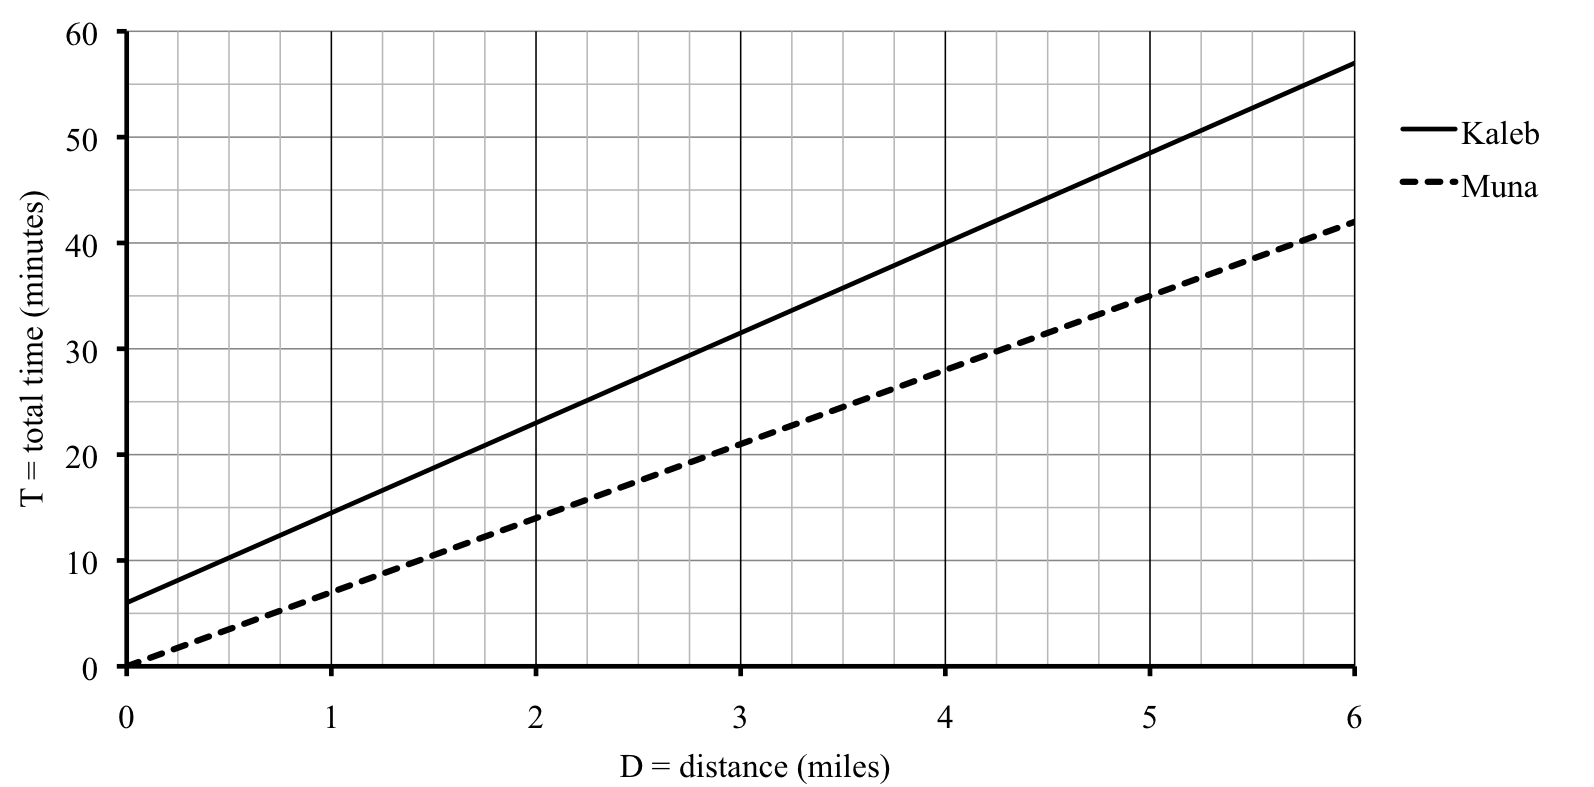
\includegraphics [width = 6in] {runtimes.png}}
\end{center}

By the way, Muna's equation $T = 7D$ is a \textbf{direct proportionality} because the only thing happening is that the independent variable is being scaled by a \textbf{proportionality constant}, $k=7$.  Any  direct proportionality fits this template.

\bigskip
 \framebox{
 \begin{minipage}[c]{.85\textwidth}  
~ \bigskip \\  \textsc{Direct proportionality template:} \quad $\text{dep} = k \ast \text{indep}$\\ ~ \bigskip
\end{minipage}
}
\bigskip

To understand the proportionality, recall that Muna can run 2.8 miles in 19.6 minutes.  What happens if she goes for a run twice as long?  Then she would be running
$2 \times 2.8 = 5.6$ miles.  Her time would be 
$$T = 7 \ast 5.6 = 7 \times \underline{5.6} = 39.2 \text{ minutes}$$
Notice that $2 \times 19.6 = 39.2$.  So, it would take her twice the time to run twice the distance.  This general idea -- that you get twice the value of the dependent variable if you have twice the value of the independent variable -- characterizes direct proportions.  We sometimes say that Muna's time is \textbf{proportional} to how far she runs.  Nothing special about twice here, as it would take her three times the time to run three times the distance, etc.

Not so for Kaleb. Remember it takes him 29.8 minutes to run that 2.8 miles.   If he runs twice the distance, which is 5.6 miles, it takes 
$$T = 6+8.5 \ast 5.6 = 6+ 8.5 \times \underline{5.6} = 53.6 \text{ minutes}$$
which is not quite twice the time, since $2 \times 29.8 = 59.6 \text{ minutes}$.
The key is that Kaleb does not stretch twice, only once, for the longer run so double the distance does not count the 6 minutes again.  Kaleb's equation is not a direct proportionality.  Another way to say that is that Kaleb's time is not proportional to how far he runs.  It is a function of how far he runs, yes, but not proportionally so.

 %\section{Intercepts and direct proportionality}

 \begin{center}
\line(1,0){300} %\line(1,0){250}
\end{center}

\section*{Homework}

\noindent \textbf{Start by doing Practice exercises \#1-4 in the workbook.}

\bigskip

\noindent \textbf{Do you know \ldots}

\begin{itemize} 
\item What the intercept of a linear function means in the story and what it tells us about the graph? 
\item How to calculate the intercept given the slope and an example (another point on the graph)? 
\item Why an intercept might not make sense, for example if it's outside the domain of the function? 
\item When a linear function is a direct proportion? 
\item Why you cannot reason proportionally if the linear function is not a direct proportion? 
\item What the graph of a direct proportion looks like? 
 \item[~] \textbf{If you're not sure, work the rest of exercises and then return to these questions.  Or, ask your instructor or a classmate for help.}
\end{itemize}

\subsection*{Exercises}

\begin{enumerate} 
\setcounter{enumi}{4}

\item Different runners run at different paces.  And take a different amount of extra time to warm-up and/or cool down. The table lists six runners, their training time to run a 5K (rounded to the nearest minute), and their pace (in minutes per mile).  
\begin{center}
\begin{tabular} {|c| |c  |c |c |c |c |c|}\hline
Name & Yannick & Olga & Aziz & Hitomi & Galen & Fiona\\ \hline
Pace & 8.2 & 8.6 & 9.5 & 10 & 10 & 11.2 \\ \hline
5K time & 32 & 35 & 33 & 36 & 31 & 44 \\ \hline
extra time & ? & ? & ? & ? & ? & ? \\ \hline
\end{tabular}
\end{center}
\begin{enumerate}
\item We are interested in each runner's extra time, but first convert 5K, which is short for 5 kilometers, to miles using $1 \text{ mile} \approx 1.609 \text{ kilometers}$.
\item Now, determine the extra (warm up/cool down) time for each runner and list your answer in the table.  Report your answer to the nearest minute.
\item List the runners in order from least to most warm up/cool down time.
\end{enumerate}

\item At 10:00 a.m.\ we've got snowy skies and 4 inches of new snow on the ground.  It's coming down fast out there at \nicefrac{2}{3} of an inch per hour.
\begin{enumerate}
\item Name the variables, measuring time in hours since 10:00 a.m.  
\item Write an equation illustrating the dependence.
\item When did the snowstorm start?
\item Name a new variable for time measured this time in hours since the snowstorm started.  
\item Write an equation illustrating the dependence using this new variable instead.  
\item Check that this equation confirms 4 inches of new snow at 10:00 a.m.
\item Explain why the two equations have different intercepts.
\end{enumerate}

\item The public beach near Paloma's house has lost about 3'9" feet a year of beach depth (measured from the dunes to the high water mark) due to erosion since they started keeping records 60 years ago.  Currently it's 210 feet deep.    

\hfill \emph{Story also appears in 1.3 Exercises}
\begin{enumerate}
\item The county is considering filling in sand to offset the erosion, back to the historical mark (60 years ago).  How deep was it then? Notice that you need to convert 3'9" to (decimal) feet first.
\item Name the variables and write an equation relating them, assuming the county does not fill in the beach now.  Measure time from 60 years ago.
\item  The country agrees to start filling in sand when the depth drops below 180 feet.  How many (more) years will that take to happen?  First estimate the answer using successive approximation.  Then set up and solve an inequality to find the answer.
\item Draw a graph showing the sand erosion over the past 60 years and including the next 20 years, assuming the county does not do any filling.
\item Identify the slope and intercept and explain their meaning in the story.
\end{enumerate}  

\item Clyde is loading bricks weighing 4.5 pounds each onto his wheelbarrow.  The wheelbarrow weighs 89 pounds when it has 16 bricks in it. (That weight includes both the bricks and the wheelbarrow itself.)
\begin{enumerate}
\item How much would Clyde's wheelbarrow weigh if it were empty?
\item Name the variables and write an equation relating them.
\item How much (total) will the wheelbarrow weigh if he loads a total of 30 bricks?
\item Clyde continues loading bricks until the wheelbarrow full of bricks weighs 206 pounds.  How many bricks are in it?
\item Graph and check.
\end{enumerate}

\item The city offers bus ``convenience'' passes -- 20 rides for \$12.95 or 80 rides for \$51.80.  
\begin{enumerate}
\item Calculate the rate of change.
\item Is there a convenience charge?
\item What is the name for this type of function?
\end{enumerate}

\item To make cookies it takes a few minutes to prepare the dough.  After that it takes 12 minutes per batch to bake in the oven.  Last time I made 3 batches of cookies and it took a total of 54 minutes. 
\begin{enumerate}
\item How long does it take me to prepare the dough?
\item How long would it take me to make 10 batches of cookies for the cookie swap?  Assume the time to prepare the dough remains the same and only one batch bakes in the oven at a time.
\item Name the variables and write an equation describing the function.
\item Identify the slope and intercept and explain their meaning in the story.
\end{enumerate}

\end{enumerate}

